\documentclass{article}
\usepackage{amsmath}
\usepackage{graphicx}
\usepackage{natbib} % Or biblatex
\usepackage{hyperref}
\usepackage{times}

\begin{document}

\title{Dual Reinforcement Learning Data Flow Summary}
\author{Vignesh Rangaraj}
\date{April 12, 2025}

\maketitle

\section{Summary}

This document summarizes the data flow in the Dual Reinforcement Learning (DRL) framework. The DRL framework is designed to optimize decision-making processes by leveraging dual learning principles.
Here we make use of two distinct learning environments: secondary and tertiary. The tertiary environment makes decisions at a higher level based on cost reward signals that collect data from BESS and DER systems.
We use the IEEE-34 bus system as a test case to demonstrate the RL agent to learn and optimize cost signals from multiple DER systems and a single BESS system. 

\section{Novelty}
To the best of my ability, these concepts have not be exploited yet in other research papers. The work makes the following contributions:

\begin{itemize}
    \item A novel dual reinforcement learning framework that integrates secondary and tertiary learning environments.
    \item A comprehensive evaluation of the DRL framework using the IEEE-34 bus system as a test case.
    \item Secondary RL agents that can provide feedback to the tertiary RL agent, allowing for a cooperative learning process.
\end{itemize}

\section{System Architecture}

As shown in Figure \ref{fig:dual_rl_architecture}, the DRL framework consists of two main components: the secondary environment and the 
tertiary environment. The secondary environment focuses on fine-grained control of inverter-based DERs, while the tertiary environment provides macro-level control over microgrids. 
The set up hopefully allows for two practical applications: (1) tertiary agent can learn not to overload the secondary agent over cost by sending in enormous amount of energy by closing the tie point
and (2) secondary agent can learn to handle the influx of energy by controlling the reactive power which has direct impact on the voltage levels. As an initial step, I am using SAC agent for
the tertiary environment and IA3C agent for the secondary environemnt. From previous research, we have already shown that SAC is suitable for continuous action space and IA3C is suitable for discrete action space..


\begin{figure}[h!]
    \centering
    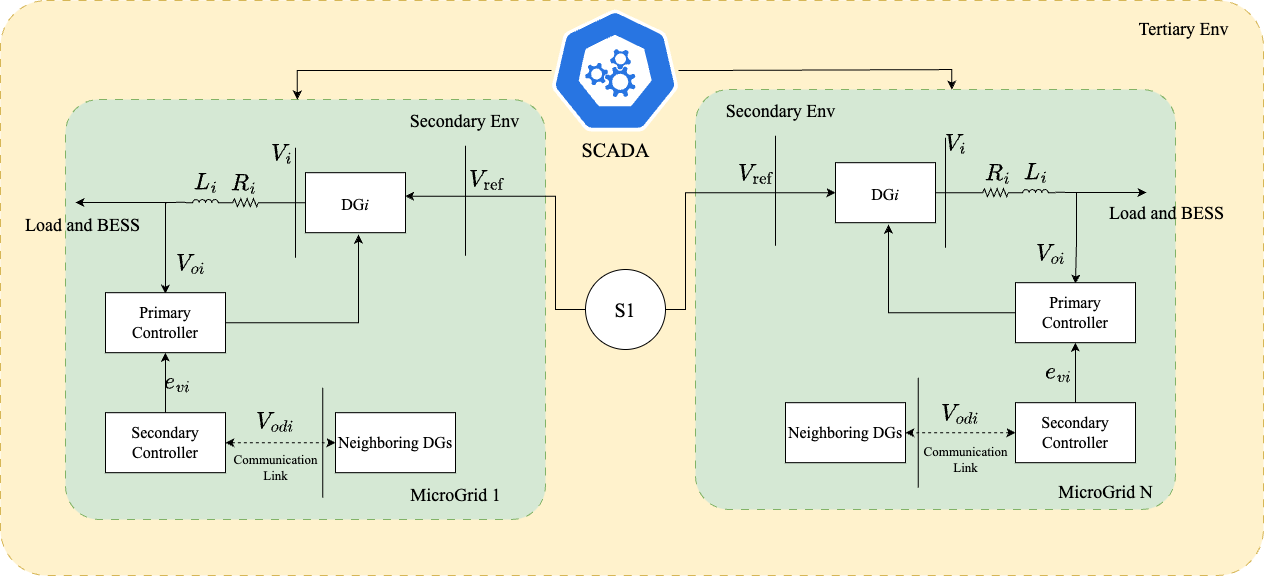
\includegraphics[width=0.9\textwidth]{dual_rl.png}
    \caption{Block diagram of the Dual Reinforcement Learning architecture showing the tertiary environment (macro control over microgrids) and secondary environment (fine-grained voltage control using inverter-based DERs).}
    \label{fig:dual_rl_architecture}
\end{figure}

\section{Code}
The code for the Dual-RL framework is here: https://github.com/vigneshrangaraj/dual-rl-fractal-grid

\section{Next Steps}
The next steps in this research include:
\begin{itemize}
    \item Simulations to ensure convergence of the applications
    \item Exploration of additional learning algorithms and architectures to enhance the performance of the DRL framework.
\end{itemize}

\end{document}